\documentclass{standalone}
\usepackage[dvipsnames,svgnames,x11names]{xcolor}
\usepackage{tikz}
\usepackage{pgfplots}
\pgfplotsset{compat = 1.12}
\usepackage{../thesismath}
\begin{document}
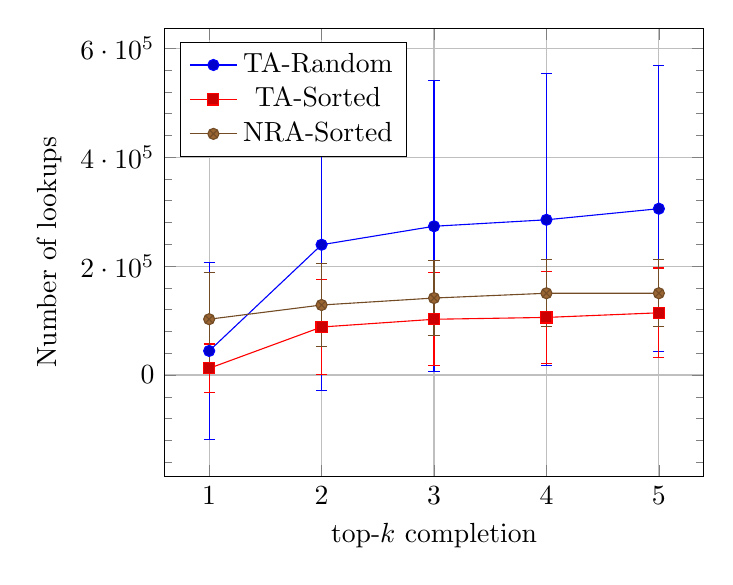
\begin{tikzpicture}[baseline]

\begin{axis}[
  xlabel = {top-$k$ completion},
  xtick = {1, ..., 5},
  ylabel = {Number of lookups},
  scaled ticks = false,
  %y tick label style={/pgf/number format/fixed},
  %ymin = -150000,
  %ymax = 1300000,
  minor y tick num = 4,
  grid = major,
  legend entries = {{TA-Random}, {TA-Sorted}, {NRA-Sorted}},
  legend pos = north west,
]

% over 100 test sequences on my own machine

% TA-MKN-Random
\addplot+[
  error bars/.cd,
  y dir = both,
  y explicit,
] table [y error = num_error] {
  n num      num_error
  1   44209  162035
  2  239249  267262
  3  273176  267049
  4  285058  268102
  5  305410  262817
};

% TA-MKN-Sorted
\addplot+[
  error bars/.cd,
  y dir = both,
  y explicit,
] table [y error = num_error] {
  n num      num_error
  1   12289   44709
  2   88165   86648
  3  102377   85678
  4  105772   84910
  5  114247   82368
};

% NRA-MKN-Sorted
\addplot+[
  error bars/.cd,
  y dir = both,
  y explicit,
] table [y error = num_error] {
  n num      num_error
  1  102508   85790
  2  128574   76631
  3  141360   68952
  4  150147   61572
  5  150222   61602
};

\end{axis}

\end{tikzpicture}
\end{document}
